\chapter{Motion}
% This chapter describes the systems governing the motion of the robot, such as leg motion planning and gait generation.
The basic operation of the motion system is as follows, first the robot is commanded to walk in a certain direction, at a
certain speed and body height. These commands are sent from the base station to Jetson Nano on the robot,
the motion controller node on the Jetson Nano then sends these commands to the gait state machine node, at a fixed frequency.
The gait state machine uses the received direction stride length to generate leg states (swinging or supporting) and the ideal
final position of each foot. These states and positions are sent back to the motion controller node where the positions are adjusted
based on the heightmap data to ensure stable footing. The leg states and adjusted feet positions are then sent to the servo 
controller node, this node controls the servos to move the robots feet to their final positions, either in a arc or linearly,
depending on their state (swinging or supporting). %A high level diagram of the motion system can be seen in \ref{fig:motion_system}.

\begin{figure}[h]
    \centering
    % \hspace{-1.38cm}
    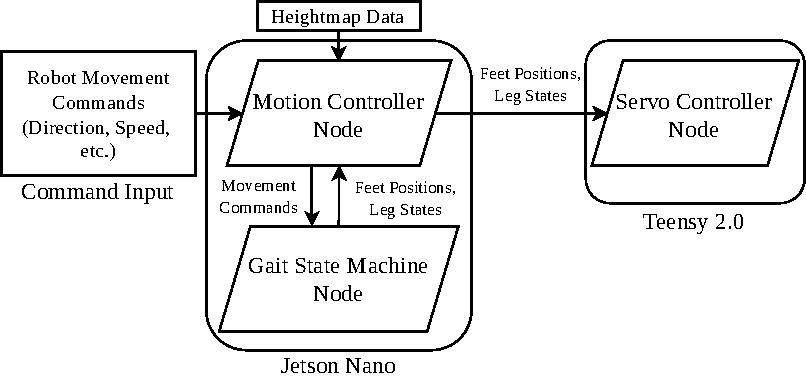
\includegraphics{Diagrams-MotionSystem.drawio.pdf}
    \caption{Motion System Overview}
    \label{fig:motion_system}
\end{figure}

\section{Gait State Machine}
The state machine used to realise the tripod gait used in the robot is quite simple, comprised of only two states, stepping and
resting, as can be seen from figure \ref{fig:gaitSM}. Table \ref{tab:state_defs} defines the actions that should be taken during
each state.

The primary computation done by this state machine is calculating which legs are supporting and which are swinging, which occurs
on entering the "Stepping" state. This function is described in section \ref{sec:supp_swing_calc}.

\begin{figure}[h]
    \centering
    % \hspace{-1.38cm}
    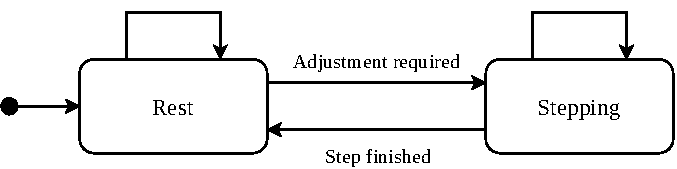
\includegraphics{Diagrams-GaitSM.drawio.pdf}
    \caption{Gait State Machine}
    \label{fig:gaitSM}
\end{figure}

\begin{table}[h]
    \center
    \begin{tabularx}{\textwidth}{|l|X|}
        \hline
        \multicolumn{2}{|c|}{Rest State Definition} \\
        \hline
        Enter Condition & Is the current step finished? \\
        \hline
        On Entering & Set all leg states as supporting. \\
        \hline
        While Active & Do nothing \\
        \hline
    \end{tabularx}
    
    \bigskip
    \noindent
    \begin{tabularx}{\textwidth}{|l|X|}
        \hline
        \multicolumn{2}{|c|}{Stepping State Definition} \\
        \hline
        Enter Condition & Is there a mismatch between feet targets and current position? \\
        \hline
        On Entering & Calculate and set the leg states based on walking direction. \\
        \hline
        While Active & Adjust feet targets based on direction, stride length and robot height\\
        \hline
    \end{tabularx}
    \caption{State Definitions}
    \label{tab:state_defs}
\end{table}

\newpage
\subsection{Choosing The Supporting And Swinging Legs} \label{sec:supp_swing_calc}
    The robot body is divided up into sextants, centered around the nominal leg positions. When calculating
    the swinging legs it is first determined in which sextant the movement direction vector falls, this is called the active sextant.
    The leg related with the active sextant, and the two opposite, are then chosen as swinging, with the remaining three legs chosen as supporting.

    The swinging legs are defined by the boolean array, \(\boldsymbol{S_i}\), as described in equation \ref{eq:is_swing}.
    \begin{equation}\label{eq:is_swing}
        \begin{gathered}
            \boldsymbol{S}_{\boldsymbol{i} - \xi} \iff i \text{ is even} \\
            \boldsymbol{S}_{\boldsymbol{i} - \xi}={i|(i-\xi) \text{ is even}} \\
            \text{Where \(i \in [0,5]\) and \(\xi\) is the active sextant/leg number.}
        \end{gathered}
    \end{equation}

    \noindent
    Figure \ref{fig:sextants} illustrates and example with sextant 2 being active. Thus legs 2, 4 and 6 are swinging, while legs 1,3 and 5 are supporting.
    \begin{figure}[h]
        \centering
        \hspace{1.1cm}
        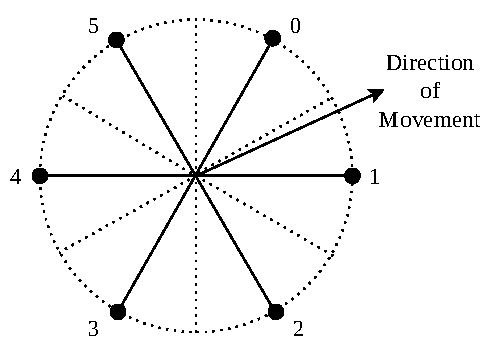
\includegraphics{Diagrams-Sextants.drawio.pdf}
        \caption{Leg sextants, with sextant 2 being active.} 
        \label{fig:sextants}
    \end{figure}

    This of course would not be sufficient to define a walking gait, as at the end of each step \(\boldsymbol{S_i}\) does not invert.
    Thus and additional step after equation \ref{eq:is_swing} is added. The current horizontal length of leg \(\xi\), defined as \(l_\xi\), is compared to its nominal
    horizontal length, \(L_\xi\). If \(l_\xi\ > L_\xi\), invert \(\xi\). As shown in equation \ref{eq:negate_is_swing}.

    \begin{equation} \label{eq:negate_is_swing}
        \begin{gathered}
            l_\xi\ > L_\xi \longrightarrow \boldsymbol{S_i} \Longleftarrow  \lnot \boldsymbol{S_i} \\
            \boldsymbol{S}_{\boldsymbol{i} - \xi} =
                                                \begin{cases}
                                                    \boldsymbol{i} \setminus \boldsymbol{S}_{\boldsymbol{i} - \xi} & l_\xi > L_\xi \\
                                                    \boldsymbol{S}_{\boldsymbol{i} - \xi} & l_\xi \leq L_\xi
                                                \end{cases}\\
            \text{Where \(i \in [0,5]\) and \(\xi\) is the active sextant/leg number.}
        \end{gathered}
    \end{equation}

\newpage
\section{Kinematics}
    When commanding a foot position, the servo controller requires a function to calculate servo angles. While the foot arc planner, see section 
    \ref{sec:arc_generation}, requires the current position of the feet to function. The \ac{ik} and \ac{fk} functions described in this section provide
    this functionality. Figure \ref{fig:kinematics} illustrates the leg geometry and variables used in the \ac{ik} and \ac{fk} functions.
    \begin{figure}[h]
        \centering
        % \hspace{-1.38cm}
        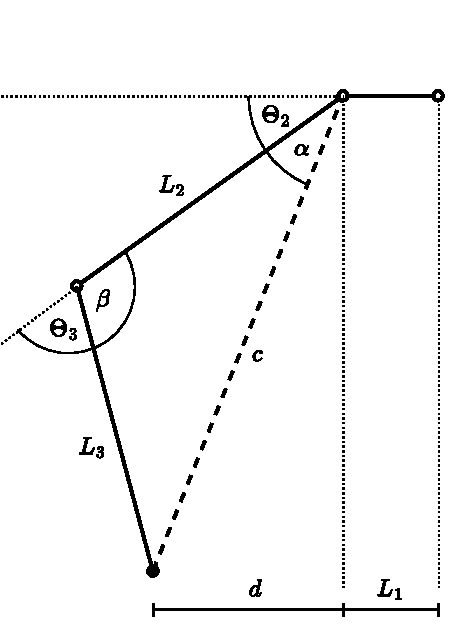
\includegraphics[clip, trim=0 0cm 0 1.51cm]{kinematics.drawio.pdf}
        \caption{Leg Kinematics Diagram}
        \label{fig:kinematics}
    \end{figure}

    \subsection{\acf{ik}}
        The \ac{ik} function calculates the leg servo angles, \(\boldsymbol{\Theta} = [\Theta_1, \Theta_2, \Theta_3]^T_{\displaystyle ,}\) required
        to move the foot to the given target position vector, \(\boldsymbol{p_t} = [x_t,y_t,z_t]^T_{\displaystyle .}\)
        \hbox{Equation \ref{eq:ik}} describes the \ac{ik} function.
        \begin{equation}\label{eq:ik}
            \boldsymbol{\Theta} =
                                \begin{bmatrix}
                                    \Theta_1\\
                                    \Theta_2\\
                                    \Theta_3
                                \end{bmatrix}
                                =
                                \begin{bmatrix}
                                    \arctan{\left(\dfrac{x_t}{y_t}\right)}\\[0.5cm]
                                    \dfrac{\pi}{4} - \alpha - \arctan{\left(\dfrac{y}{d-L_1}\right)}\\[0.5cm]
                                    \dfrac{\pi}{2} - \beta
                                \end{bmatrix}
        \end{equation}
        Where \(\alpha\), \(\beta\), \(c\) and \(d\) are calculate as shown in equations \ref{eq:alpha} to \ref{eq:dik}.
        \begin{align}
            \alpha &= \arcsin{\left(\frac{L_3\sin{\beta}}{c}\right)} \label{eq:alpha} \\
            \beta &= \arccos{\left(\dfrac{L_1^2 + L_2^2 -c^2}{2L_1L_2}\right)}\\
            c &= \sqrt{(d-L_1)^2+z_t^2}\\
            d &= \sqrt{x_t^2 + y_t^2} \label{eq:dik}
        \end{align}
    \subsection{\acf{fk}}
        The \ac{fk} function calculates the position vector of a foot, \(\boldsymbol{p_c} = [x_c,y_c,z_c]\),
        given the current angles of the leg servos, \(\boldsymbol{\theta} = [\theta_1, \theta_2, \theta_3]\).
        \begin{align}
            \boldsymbol{p_c} =
                            \begin{bmatrix}
                                x_c\\
                                y_c\\
                                z_c
                            \end{bmatrix}
                            =
                            \begin{bmatrix}
                                d\cos{\theta_1}\\
                                d\sin{\theta_1}\\
                                L_2\sin{\theta_2} + L_3\sin{\left(\theta_2 + \theta_3\right)}
                            \end{bmatrix}
        \end{align}
        Where \(d\) is calculated as shown in in equation \ref{eq:dfk}.
        \begin{equation}\label{eq:dfk}
            d = L1 + L_2\sin{\theta_2} + L_3\sin{(\theta_2 + \theta_3)}
        \end{equation}
    
    \subsection{Angular Rate}
    To move a foot on a desired path it is important to not only know the absolute angle of the three leg servos, but also the angular rates of all three
    servos. If the servos are all moved at the same rate, the shape of the path that the foot follows will not be linear, but rather dependant on the
    current foot position. This is undesirable, thus equations \ref{eq:rate} define the derivative of the \ac{ik} equations (\ref{eq:ik}), i.e. the angular
    rate.

    \begin{equation}\label{eq:rate}
        \boldsymbol{\omega} =
                            \begin{bmatrix}
                                \omega_1\\
                                \omega_2\\
                                \omega_3
                            \end{bmatrix}
                            =
                            \begin{bmatrix}
                                \displaystyle \frac{- x\dot{y} + y \dot{x}}{x^2 + y^2}\\[0.5cm]
                                \dfrac{\pi}{4} - \alpha' - \arctan{\left(\dfrac{y}{d-L_1}\right)}\\[0.5cm]
                                \dfrac{\pi}{2} - \beta'
                            \end{bmatrix}
    \end{equation}

\newpage
\section{Foot Motion} \label{sec:arc_generation}
    When taking a step the foot can not simply be moved to its destination in a straight line, as doing so will cause the foot to be dragged on the terrain,
    impeding the movement of the robot. Thus it is required to move the foot in an arc like motion to clear any obstacles that might be in its path.

    \subsection{Existing System}
        The existing system will, at the start of each step, compute an arc for each foot to follow, this arc is then sent to the servo controller
        to be executed. While efficient and effective in ideal conditions, this method of defining the arc has poor performance when considering external
        influences. If for example the robot has to adjust the final target of its feet mid step, this arc would have to be recomputed in its entirety,
        thus leading to possible performance concerns.

        In addition to this Text, the current system is designed with the assumption that the starting position of the foot is grounded, thus if the arc is recomputed
        mid step the arc will be undesirable, as it will rise with the desired step height for a second time. This is illustrated in Figure \ref{fig:old_arc}.

        \begin{figure}[h]
            \centering
            \hspace{-1.38cm}
            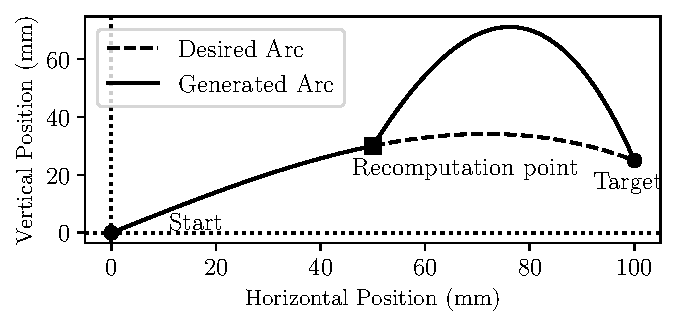
\includegraphics{old_path.pdf}
            \caption{Existing arc recomputation problem}
            \label{fig:old_arc}
        \end{figure}

    \subsection{Improved System}
        The improved system solves this problem by utilising a flow function. During a step, this function will continuously calculate the
        direction that the foot must move to reach its destination. Thus this system is resilient to external disturbances and is capable of adjusting to
        varying destination and step height requirements. 
        
        The flow field is designed to first move the foot vertically upwards until horizontal coplanar with the destination, and then to follow a
        arc to the destination with a defined step height, this can be adjusted to make the arc start before or after coplanar. The step height can be adjusted at any point in time and the flow field will adjust accordingly.
        Figure \ref{fig:foot_arc} illustrates the field function and is described in section \ref{sec:flow_function}.
        \begin{figure}[h]
            \centering
            \hspace{-1.38cm}
            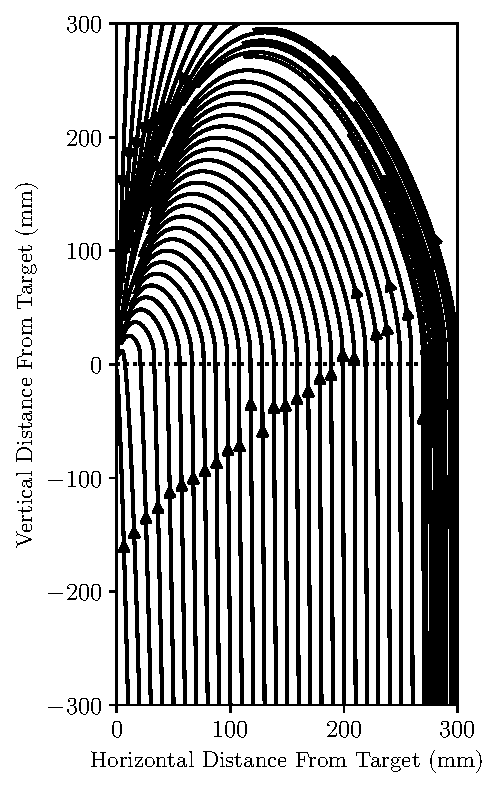
\includegraphics{foot_path.pdf}
            \caption{End effector movement path}
            \label{fig:foot_arc}
        \end{figure}

        \subsubsection{Flow Function Description} \label{sec:flow_function}
            The flow function, \(\rho(x,y)\), uses the gradient function of a parabola passing through the point \([0,0]\) and \([x,y]\) as a basis, where point \([x,y]\)
            is the current point that is being evaluated and \(x\) is the horizontal distance between the destination and the current point and \(y\) the
            vertical distance. The final function is described by equations \ref{eq:rho} to \ref{eq:sigmoid}, for the process of designing the flow function
            please see appendix \ref{app:flow_function}.
            \begin{equation} \label{eq:rho}
                \begin{aligned}
                    \rho(x,y) &= \frac{\delta}{\delta x\delta y}&&f_a(x,y)x^2 + f_b(x,y)x + C\\
                    &= &&2f_a'(x,y) + f_b'(x,y)    
                \end{aligned}
            \end{equation}
            Where \(f_a'(x,y)\) and \(f_b'(x,y)\) are defined as follows:
            \begin{align} \label{eq:fa}
                f_a'(x,y) &= -\left|\frac{v_h}{x}\right| - \left|S(y)\right|\\
                f_b'(x,y) &= \frac{y}{x} - f_a(x,y)
            \end{align}
            Where \(v_h\) is the variable describing the step height and \(S(y)\) is a sigmoid like function defined in Equation \ref{eq:sigmoid}.
            \begin{equation} \label{eq:sigmoid}
                S(y) = \frac{0.6(y-q)}{1+\left|y-q\right|-0.59}
            \end{equation}
            Where \(q\) is the variable that determines at which vertical displacement the leg path transitions from primarily an vertical motion to
            an arc motion.






